% -*- coding: utf-8; -*-

\chapter{Processo de Restauração de Seções Geológicas}

\section{Sistema Recon MS}

\subsection{Introdução}

O ambiente no qual este trabalho é desenvolvido é o \textit{Sistema Recon MS}, um software amplamente usado dentro da indústria de óleo e gás pela Petrobras e capaz de auxiliar na restauração de modelos geológicas.\cite{ReconTecgraf} Conta com editor gráfico, estruturas de dados topológicos, algoritmos de transformações geológicas, gráficos de pós-processamentos entre outros recursos.

O Sistema Recon é desenvolvido a partir de um convênio entre o Instituto Tecgraf/PUC-Rio e a Petrobras desde 1991. Atualmente sua equipe responsável é formada pelo Grupo de Modelagem Digital em Geociências do Tecgraf. Uma imagem (Figura~\ref{fig-recon}) da tela inicial do programa é mostrada abaixo.

\begin{figure} [H]
  \begin{center}
    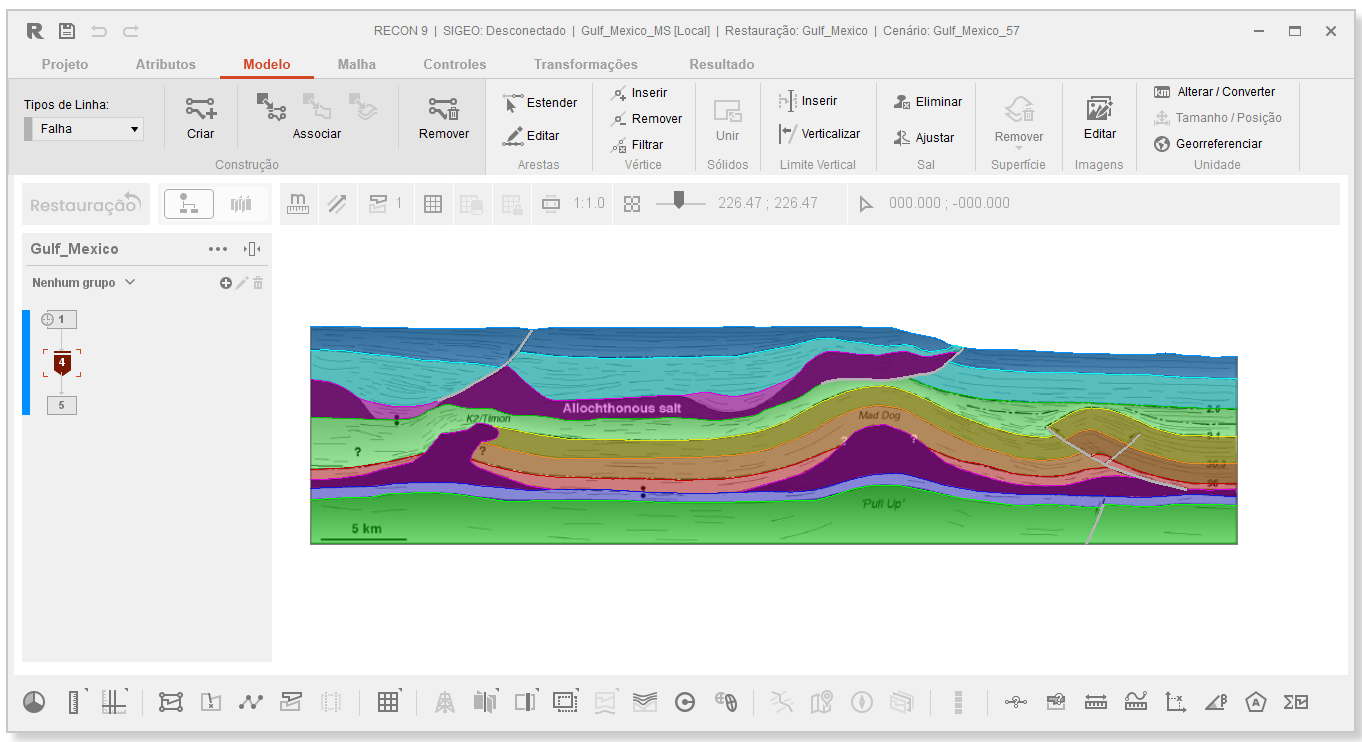
\includegraphics[width=\textwidth]{images/fig-recon}
    \caption{Captura de tela do Sistema Recon MS\cite{Recon}.}\label{fig-recon}
  \end{center}
\end{figure}

A restauração de seções geológicas pode ser entendida como uma manipulação da seção a fim de realizar a reconstituição dela ao seu estado anterior às deformações ocorridas ao longo do tempo, em outras palavras busca-se realizar uma retrodeformação na seção e assim usar na interpretação estrutural de uma região de interesse.\cite{Fossen}

Neste capítulo são apresentadas as principais características do Sistema Recon MS para o objeto deste trabalho a fim de prover uma contextualização para o que é exibido nos demais capítulos. As próximas subseções tratam da descrição dos componentes principais e recursos básicos disponibilizados pelo programa no processo de restauração de seções geológicas e também de visualização tridimensional do modelo. 

\subsection{Subdivisão Planar} % Falar do HED e da TopS

Uma seção geológica pode ter sua representação digital como uma subdivisão planar uma vez que ela pode ser vista como um conjunto de polígonos que dividem o domínio da seção. Estes polígonos podem sofrer deformações e deslocamentos oriundos das transformações geológicos às quais a seção pode sofrer durante o balanceamento. Há ainda informações de adjacências entres essas porções que também precisam ser consideradas em um contexto computacional da seção geológica.

Na Figura~\ref{fig-subdivisao-planar} é possível perceber, por exemplo, que as camadas A, B e C possuem 3 blocos separados por falhas. Cada bloco é uma região fechada delimitada por um conjunto de segmentos. Deve-se observar ainda que essas regiões possuem atributos geológicos como idade, litologia, porosidade, etc.

\begin{figure} [h]
  \begin{center}
    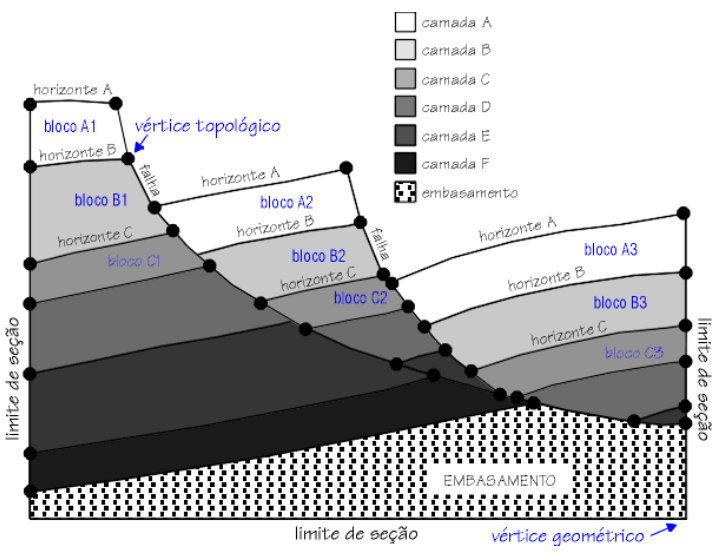
\includegraphics[width=400pt]{images/fig-subdivisao-planar}
    \caption{Seção geológica como uma subdivisão planar.\cite{Ferraz}}\label{fig-subdivisao-planar}
  \end{center}
\end{figure}

Uma subdivisão planar pode ser definida como uma subdivisão do plano através do uso de \textit{arestas}, \textit{vértices} e \textit{faces}.\cite{Berg} Essas são as entidades topológicas presentes em uma subdivisão planar, a face é como a região descrita anteriormente, delimitada por arestas (segmentos de curva); os vértices são os limites das arestas, sendo um para cada extremidade (podendo ser o mesmo vértice no início e no final da aresta).

A subdivisão planar precisa atender a alguns requisitos em relação às entidades topológicas: não deve haver vértices coincidentes; arestas só podem se cruzar em um vértice e faces também só se cruzam ou em um vértice, ou em uma aresta. Em outras palavras, não deve existir sobreposição de elementos topológicos. 

No entanto, há ainda um último componente topológico: o \textit{loop} ou \textit{laço} que é, de forma sucinta, um suconjunto conexo e ordenado de arestas. Com essa definição, a \textit{face} pode ser interpretada como uma união de laços, um deles sendo externo (delimitando a fronteira externa da face) e zero ou mais internos.

Em suma, a subdivisão planar tem os seguintes elementos topológicos:
\renewcommand{\labelitemi}{•}
\begin{itemize}
  \item \textbf{Vértice}: representa um ponto único dentro do plano.
  \item \textbf{Aresta}: segmento de curva com vértices como limites.
  \item \textbf{Laço} (loop): suconjunto conexo e ordenado de arestas.
  \item \textbf{Face}: região delimitada por um ou mais laços.
\end{itemize}

\subsection{Modelagem da Subdivisão Planar}

Para modelar a subdivisão planar dentro do Recon é utilizada a biblioteca computacional \textbf{HED} desenvolvida pelo Instituto Tecgraf/PUC-Rio que é a implementação de uma estrutura de dados topológicos baseada em arestas, a \textit{Half-Edge}, uma das razões para esta escolha são as relações fixas de adjacência que uma aresta apresenta em relação às outras componentes topológicas. Uma aresta sempre é delimitada por dois vértices (distintos ou não) e é adjacente à duas faces.\cite{HED}

O HED introduz uma nova entidade que explora bem essa característica denominada \textit{half-edge} ou \textit{semiaresta} que é uma referência ao \quotes{uso} da aresta por uma face. Dessa forma, no HED, cada aresta é formada por duas semiarestas, cada semiaresta guarda uma referência para uma face e também para um vértice de origem. Isto dá uma orientação para a semiaresta que é usada para indicar o sentido positivo do loop das faces, por exemplo.

A estrutura HED tem um aspecto hierárquico de listas duplamente encadeada de elementos topológicos. No nível mais alto está a subdivisão planar, denominada como \textit{HedSolid}, então vêm \textit{HedFace}, \textit{HedLoop}, \textit{HedHalfEdge} e \textit{HedVtx} no nível mais baixo. A representação da aresta, \textit{HedEdge} encontra-se no mesmo nível da HedHalfEdge.

Uma propriedade importante em estruturas topológicas são as relações de adjacências entre suas componentes, a HED não provê de forma direta todos as relações, contudo é possível chegar às demais com uso de indireções. Por exemplo, partindo de uma aresta, como chegar às faces vizinhas? Basta ir às semiarestas da aresta, cada semiaresta possui referência para uma face.

Apresentado o HED e seus elementos, a associação com as entidades geológicas é intuitiva. Uma camada geológica é representada por uma face; as linhas de horizonte, falha ou sal têm como correspondente as arestas, por último, cada conjunto contínuo de faces é associado a um sólido\footnote{Os sólidos representam uma subdivisão planar e em alguns casos, a seção pode apresentar partes inteiramente descontínuas onde cada uma é um sólido diferente. Para casos onde é necessário sobreposição de partes, só é possível com a existência de mais de um sólido.}.

Destaca-se que a ideia de representar a seção geológica como uma subdivisão planar, ou uma estrutura HED, visa facilitar a criação e manipulação computacional da seção durante o processo de restauração. Todavia, a representação completa precisa levar em consideração também os atributos geológicos.

\subsection{Atributos Geológicos}

Como já dito, os blocos que formam a seção geológica possuem propriedades próprias e precisam também estarem salvas na estrutura de dados topológica.

Cada entidade do HED possui um campo reservado para um tipo genérico de informações e é neste espaço que são organizados os atributos geológicos da seção. Estes atributos são representados em estruturas chamadas \textit{GeoSolid}, \textit{GeoFace}, \textit{GeoEdge} e \textit{GeoVtx}. Pela nomenclatura, é fácil observar a relação com o HED. As principais informações organizadas nessas estruturas são:

\renewcommand{\labelitemi}{•}
\begin{itemize}
  \item \textbf{GeoSolid}: o sólido por ser a estrutura mais alto nível, é quem vai guardar referência à seção e ao cenário ao qual pertence dentro da restauração.
  \item \textbf{GeoFace}: é a estrutura que precisa armazenar dados do material geológico que a compõe (como idade, tipo, características físicas, etc.) e malha de triângulos que pode ser manipulada pelas transformações.
  \item \textbf{GeoEdge}: estrutura que guarda o tipo de linha (de horizonte, falha, topo de sal, etc.) e a subdivisão geométrica que forma a linha. 
  \item \textbf{GeoVtx}: é a única que armazena apenas o identificador universal.
\end{itemize}

Aliás, todas as estruturas de atributos geológicos possuem um campo para salvar este identificador que possui o formato \textit{UUID} --- \textit{universally unique identifier} ou identificador único universal que é usado, por exemplo, na associação dos elementos geológicos com a malha triangular das faces, que será apresentada adiante.\cite{UUID}

\subsection{Seções Geológicas} % Falar da árvore de cenários

O principal recurso do Sistema Recon é seu conjunto de ferramentas para manusear uma seção geológica, desde a digitalização das informações que a definem geometricamente, da caracterização dos materiais e propriedades, da criação de dispositivos de controle e monitoramento da restauração até o kit de transformações que irão deformar a seção.

\subsubsection{Criação de uma seção geológica}

Para criar uma seção geológica no Sistema Recon pode-se recorrer ao editor gráfico para desenhar linhas e atribuir propriedades manualmente conforme seu tipo (se for horizonte, falha, limites da seção, etc.) ou em modelos que apresentem superfícies tridimensionais, como na Figura~\ref{fig-recon-1}, as seções podem ser criadas pela interseção de um plano vertical segundo uma direção dada pelo usuário, essa ação é chamada de \textit{fatiamento} do modelo.

\begin{figure} [H]
  \begin{center}
    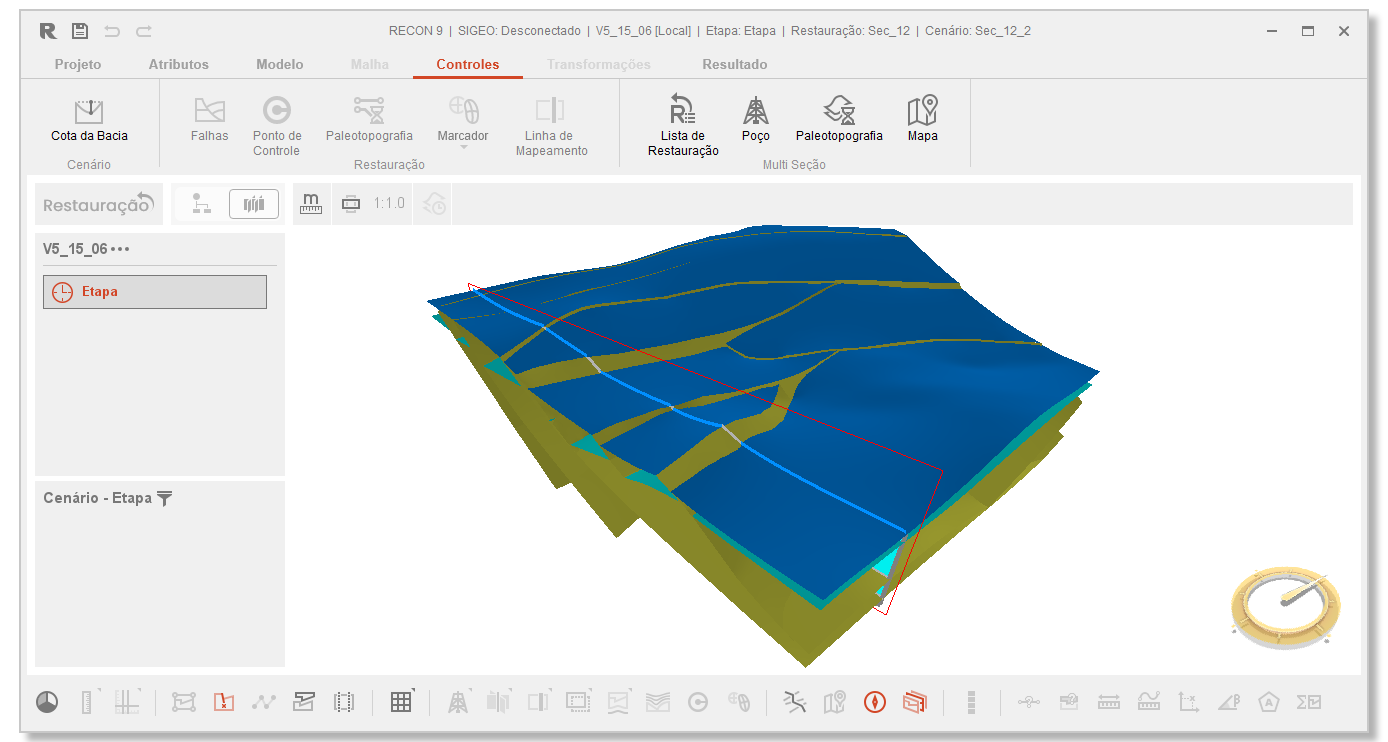
\includegraphics[width=\textwidth]{images/fig-recon-1}
    \caption{Sistema Recon exibindo um modelo com superfícies tridimensionais e uma seção em destaque.}\label{fig-recon-1}
  \end{center}
\end{figure}

Neste último caso, em especial no contexto deste trabalho, o ideal é que após a seção ter sido criada ocorra o mínimo de edição inicial nas linhas geradas. Isso é importante pois quanto melhor definida esteja a seção após o fatiamento, mais coerente com as superfícies tridimensionais estará o modelo como um todo. Edições nas linhas são comuns de acontecerem para que seja possível realizar a restauração da seção. Entretanto, em caso de edições maiores ocorrerá o descasamento entre seção e superfícies, mais tarde, no mapeamento da superfície, poderão haver incongruências.

\subsubsection{Malhas da seção geológica}

A seção geológica é representada como uma subdivisão planar, como já citado, e é utilizada a biblioteca HED na implementação dessa subdivisão. Na Figura~\ref{fig-recon-2} pode-se observar uma seção geológica e alguns elementos, como as linhas (\textit{HedEdges}) onde a sua cor representa o atributo de tipo e as faces (\textit{HedFaces}) que são, em termos simples, regiões fechadas por linhas. Neste exemplo, todas as faces pertencem à mesma camada geológica.

\begin{figure} [h]
  \begin{center}
    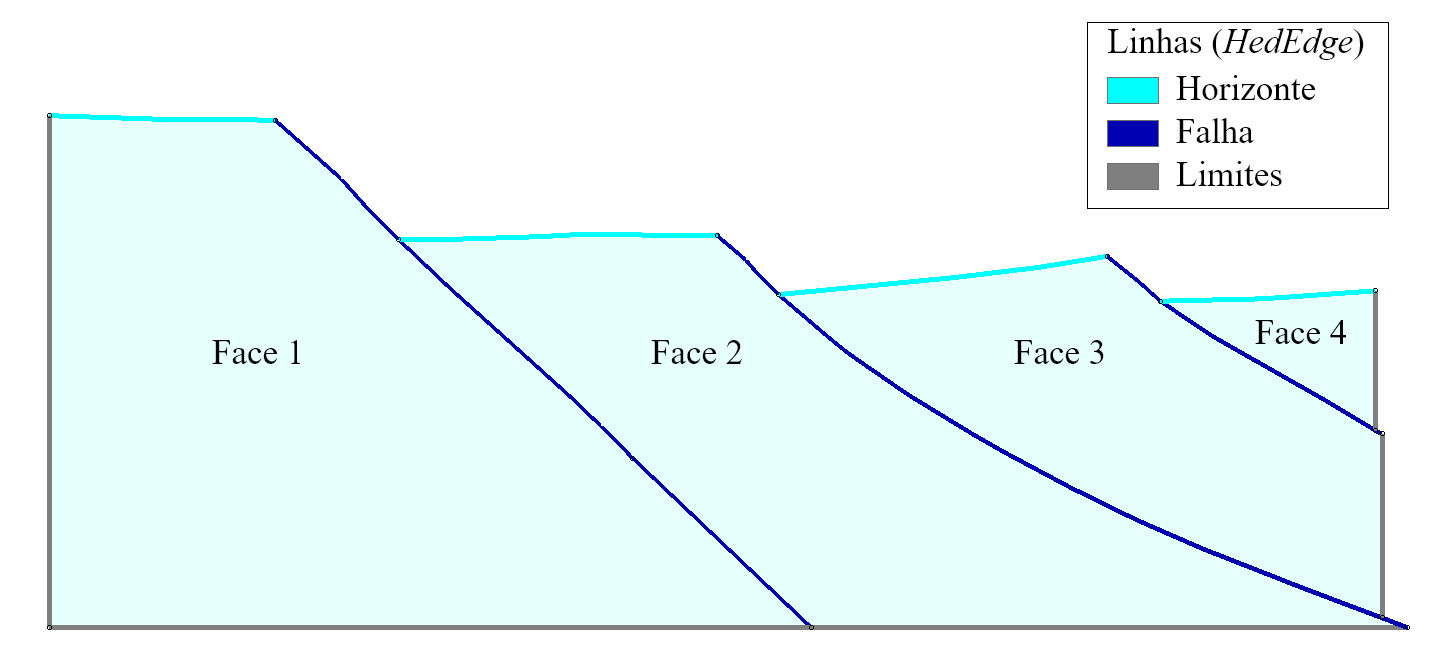
\includegraphics[width=\textwidth]{images/fig-recon-2}
    \caption{Seção geológica com destaque para os elementos de linhas e faces.}\label{fig-recon-2}
  \end{center}
\end{figure}

As faces têm um atributo muito importante para o trabalho de restauração, que são as malhas de triângulos. Cada face possui uma malha independente das outras. No Sistema Recon, essa malha é armazenada numa estrutura de dados topológicos chamada \textit{TopS} que trata-se de uma biblioteca computacional voltada para representação de malhas de elementos finitos.\cite{Tops} A Figura~\ref{fig-recon-3} exibe a mesma seção, mas com adição das malhas das faces.

\begin{figure} [H]
  \begin{center}
    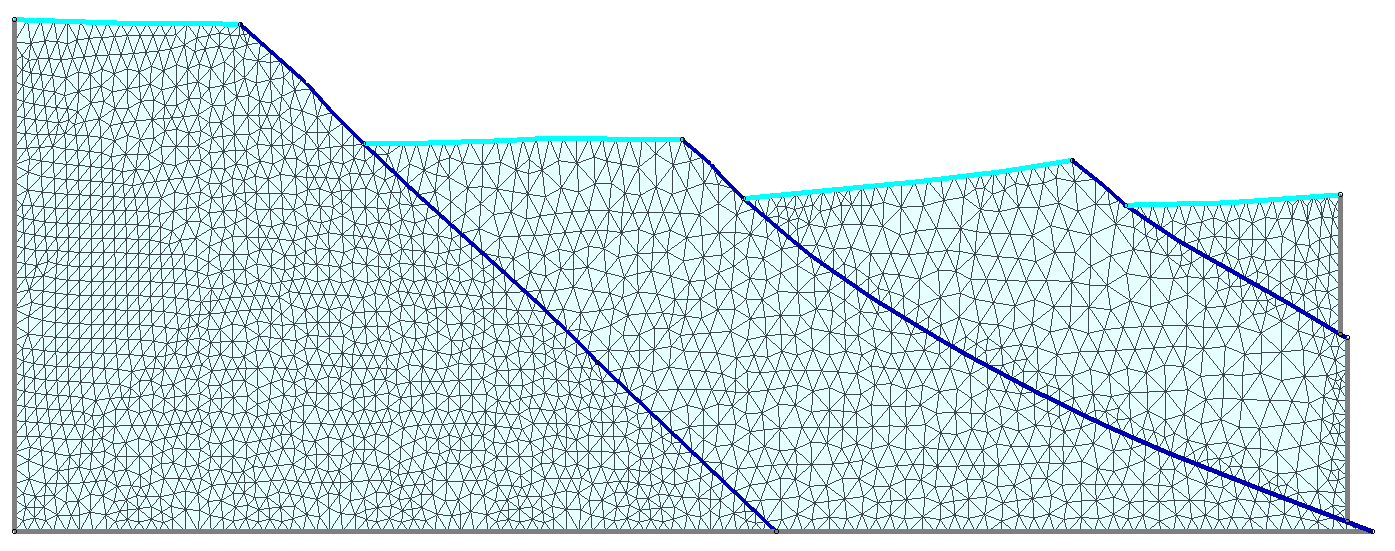
\includegraphics[width=350pt]{images/fig-recon-3}
    \caption{Malhas das faces de uma seção geológica no Sistema Recon.}\label{fig-recon-3}
  \end{center}
\end{figure}

A importância das malhas dentro da restauração de seções no Sistema Recon se dá por conta das transformações geológicas que possuem como requisito de entrada uma malha. Um pouco mais de detalhes sobre as transformações será apresentado adiante.

A estrutura \textit{TopS} permite armazenar certos atributos em seus elementos topológicos. Em especial nos vértices da malha, no Sistema Recon, é armazenado o \textit{UUID} do atributo geológico da entidade topológica do HED sobre a qual aquele vértice está, em outras palavras, se o vértice da malha está no interior da face, ele guarda o \textit{UUID} da \textit{GeoFace} dessa face, o mesmo para caso esteja sobre uma aresta (\textit{GeoEdge}) ou vértice (\textit{GeoVertex}). A Figura~\ref{fig-recon-4} mostra um exemplo da forma como esses dados são obtidos.

\begin{figure} [H]
  \begin{center}
    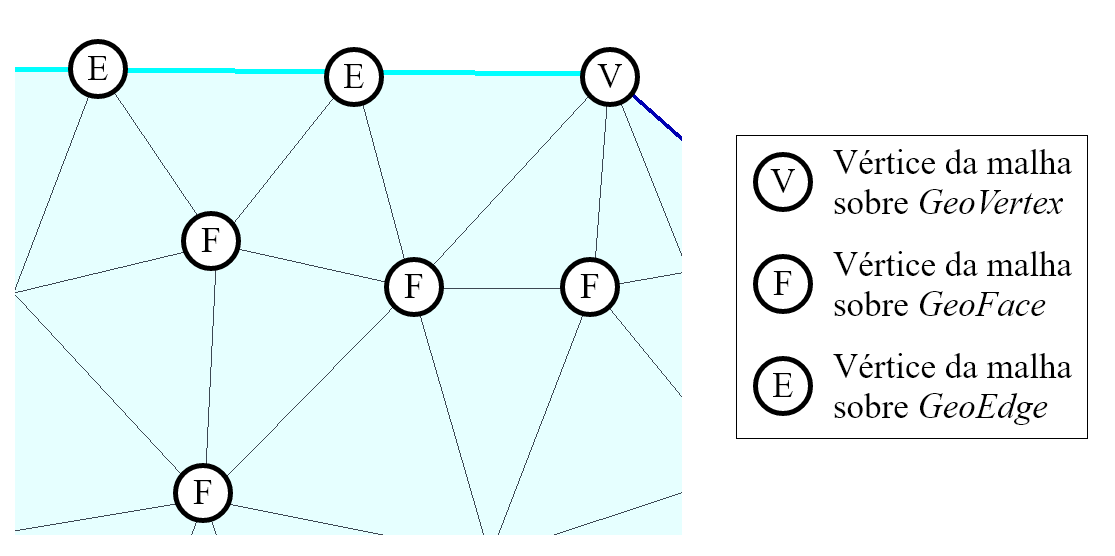
\includegraphics[width=\textwidth]{images/fig-recon-4}
    \caption{Trecho de uma malha de face com os tipos de atributo geológicos que estão sob os vértices da malha.}\label{fig-recon-4}
  \end{center}
\end{figure}

Essa relação permite identificar, a partir de um vértice da malha, sobre qual entidade geológica está este vértice, este recurso será usado no próximo capítulo.

\subsubsection{Transformações}

As transformações geológicas são ferramentas que buscam reverter (ou simular) as movimentações e deformações ocorridas aos blocos de rocha ao longo do tempo.\cite{Santi} As transformações são aplicadas diretamente às malhas, no entanto, para sua que isso aconteça, é necessário antes a definição de \textit{Módulos} na seção. 

Módulos nada mais são que agrupamentos de faces ou blocos da seção, têm o intuito de reunir aquelas partes que devem ter recebido as mesmas deformações, podendo ser, inclusive partes de camadas diferentes.

Com o módulo definido, consegue-se aplicar uma transformação. Esta irá ser empregada sobre a malha de cada uma das faces que compõem aquele módulo, deformando esta malha e, por conseguinte, alterar a geometria da seção.

A Figura~\ref{fig-recon-5} mostra a aba \quotes{Transformações} do Sistema Recon onde é possível ver os grupos de transformações e também a quantidade de opções disponíveis. Mais detalhes sobre cada uma delas podem ser consultados no manual do usuário do programa\cite{Recon}.

\begin{figure} [H]
  \begin{center}
    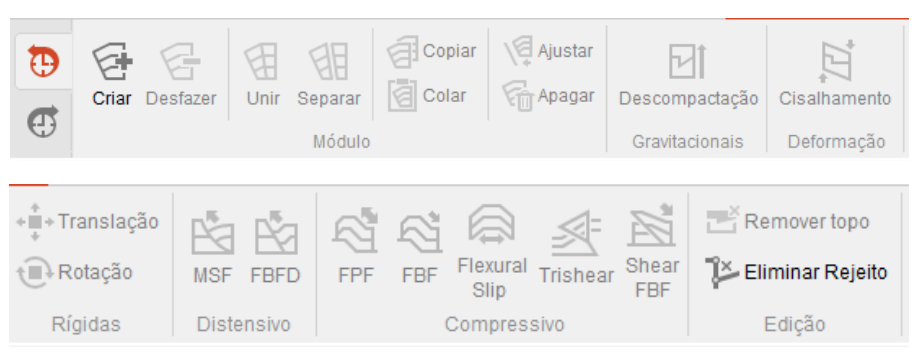
\includegraphics[width=\textwidth]{images/fig-recon-5}
    \caption{Aba \quotes{Transformações} do Sistema Recon.}\label{fig-recon-5}
  \end{center}
\end{figure}

\subsubsection{Árvore de cenários}

A restauração de seções é um processo linear no sentido de que cada novo passo depende de como estava o anterior e ainda por ser relacionado a uma escala de tempo, qualquer mudança num passo desses acarreta em um resultado diferente ao final. Além do mais, balanceamento de seções não é uma atividade de resposta única, dois geólogos podem chegar a resultados diferentes e igualmente corretos ao trabalharem com o mesmo modelo. 

Diante disto, o Sistema Recon disponibiliza em sua interface de manipulação das seções um componente capaz de registrar o histórico de etapas no processo de restauração, mais que isso, ao usuário é dado a possibilidade de voltar em algum ponto e criar uma nova linha de estudo dentro desse processo todo, ou ainda apagar uma sequência de etapas a que ele julga estar incorreta.

Isso tudo é possível graças à árvore de cenários. Um cenário é a representação de um estado de restauração de uma seção. Por exemplo, se de um passo a outro da restauração ocorre uma transformação, o estado anterior pode ser registrado em um cenário e o posterior em um outro. De cada cenário pode-se criar diversos outros como se fossem diferentes linhas do tempo, ou diferentes interpretações daquele passo de restauração.

Árvores são um tipo especial de estrutura de dados não-linear e neste casos de uso é definida como tendo uma raiz ou nó inicial que aponta para um ou mais outros nós. Estes, igualmente, podem apontar para outros diferentes nós numa escala hierárquica. A Figura~\ref{fig-recon-6} apresenta um exemplo de árvore de cenários tirada do Sistema Recon. Nesta imagem, cada quadrinho representa a seção num dado estado e como identificação, cada cenário também possui um número.

\begin{figure} [H]
  \begin{center}
    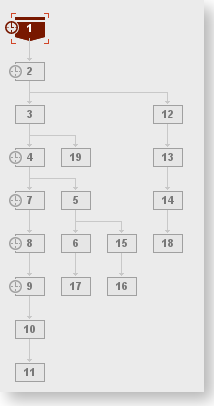
\includegraphics[width=160pt]{images/fig-recon-6}
    \caption{Exemplo de árvore de cenários de uma seção do Sistema Recon.}\label{fig-recon-6}
  \end{center}
\end{figure}

O primeiro cenário tem a seção em sua versão inicial e a cada nova manipulação da mesma, pode-se criar um novo cenário e assim ter este histórico. Essa maneira de organizar uma restauração é útil não só no contexto de uma seção isolada, mas principalmente quando se trabalha em modelos de multisseções que irão sofrer os mesmos processos de restauração, mas de maneiras diferentes. Com um registro do quê e quando ocorreu uma dada transformação em diferentes seções é possível ter uma visão mais geral do modelo em uma sequência cronológica.

\subsection{Ambiente Multisseções}

Apesar dos principais recursos do Sistema Recon sejam para se trabalhar diretamente com seção geológica, isso não significa dizer que só seja possível manipular modelos com uma única seção geológica. Uma das grandes mudanças ocorridas no programa foram a criação de ferramentas para se tratar de modelos com múltiplas seções, ou modelos multisseção.

O ambiente multisseção (MS) do Sistema Recon trata-se de um visualizador 3D onde podem ser vistas as superfícies geológicas e também as seções em um contexto global do modelo.

Como sistema de referências, o ambiente MS usa coordenadas UTM (Universal Transversa de Mercador) para localizar seus objetos. Neste sistema, cada ponto é representado por um par $(N, E)$ onde $N$ é a coordenada norte-sul em metros e $E$, a coordenada leste-oeste.\cite{IBGE}

A Figura~\ref{fig-recon-7} exibe o Sistema Recon no ambiente MS, onde é possível notar o (1) visualizador tridimensional com superfícies e seções geológicas, (2) a lista de \textit{EtapasMS} que será apresentada a seguir juntamente da (3) lista de cenários da etapa.

\begin{figure} [H]
  \begin{center}
    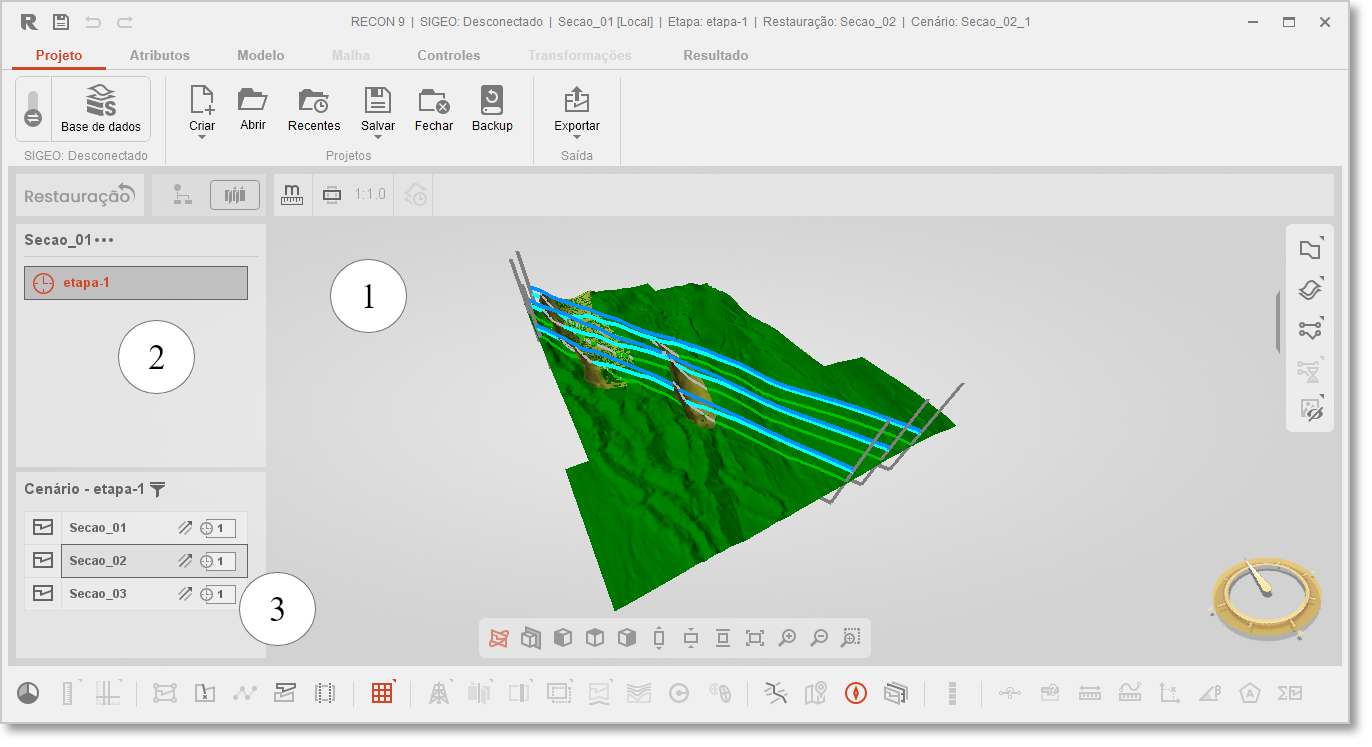
\includegraphics[width=\textwidth]{images/fig-recon-7}
    \caption{Ambiente Multisseção do Sistema Recon.}\label{fig-recon-7}
  \end{center}
\end{figure}

\subsection{Etapas de restauração}

Como brevemente apresentado, o ambiente MS permite ter uma olhar mais global do modelo e de todos os componentes que o formam. Neste contexto é então preciso organizar as seções de forma que haja o máximo de coerência do ponto de vista geral durante a restauração do modelo. Podem existir seções que compartilham uma mesma falha ou um mesmo evento tectônico, por exemplo.

Como já visto, cada seção conta com um registro de cada passo dado no andamento da restauração e é um recurso presente apenas localmente e independente. No entanto, seções relativamente próximas, ou que foram restauradas de maneira semelhante precisam sincronizar esse histórico para que haja uma ordem melhor do modelo sob um aspecto global.

Com essa finalidade, foi criado e implementado o conceito de \textit{EtapaMS} que trata-se de um conjunto de cenários de seções diferentes mas que, de certa forma, representam o mesmo marco geológico, como a restauração de uma falha ou descompactação. Cada \textit{EtapaMS} pode ter apenas 1 cenário por seção dentro de sua estrutura, isso permite ter um histórico do modelo multisseção análogo à árvore de cenário da seção individualmente.

No Sistema Recon, as \textit{EtapasMS} são dispostas em lista no ambiente multisseção. Ao selecionar um item dessa lista, logo abaixo é exibido o conjunto de cenários (por seção) que compõem aquela \textit{EtapaMS}, como bem mostra a Figura~\ref{fig-recon-7}.

Uma forma de uso das \textit{EtapasMS} para a restauração de modelos geológicos é organizar os estados de seções diferentes que respondam ao mesmo evento ou marco geológico. Caso haja uma falha X que atravessa 3 seções e em todas elas essa falha é restaurada, basta pega o cenário de cada seção onde isso ocorre e criar uma \textit{EtapaMS} correspondente a este marco. Esta organização da restauração é parte importante para o mapeamento de superfícies e volume.


